We want to numerically solve the integral equation
\[
    \int_{\partial\Omega} \big( \phi \partial_{\nhat} \ln{r} - \ln{r} \partial_{\nhat} \phi \big) \,\dee S = \pi \phi(\bzhe).
\]

\subsection{The Boundary Element Method}
We discretize the boundary with $N$ collocation points, and connect them with straight line segments $S_k$ such that
\[
    S = \bigcup_{m = 1}^{N} S_m.
\]
For convex $\Omega$, the discrete boundary $S$ will enclose a smaller area.
\begin{figure}[H]
    \centering
    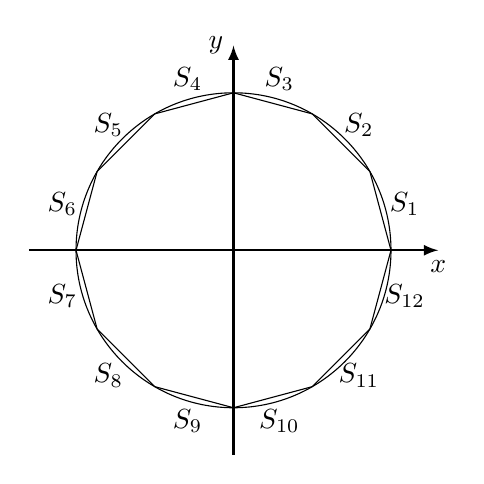
\begin{tikzpicture}
    \begin{scope}[scale = 2]
        \draw[thick, -latex] (-1.3,0)--(1.3,0) node[below]{$x$};
        \draw[thick, -latex] (0,-1.3)--(0,1.3) node[left]{$y$};
        \draw (0,0) circle (1);
        \def\angel{30}
        \foreach \x in {1,...,12}
        {
            \draw ({cos((\x-1)*\angel)}, {sin((\x-1)*\angel)})--({cos(\x*\angel)}, {sin(\x*\angel)});
            \node at ({1.125*cos((2*\x-1)*\angel/2)}, {1.125*sin((2*\x-1)*\angel/2)}) {$S_{\x}$};
        }
    \end{scope}
\end{tikzpicture}
\end{figure}
\noindent We can then set the potential function and its derivatives constant across these line segments as an approximation so that
\[
    \int_{\partial\Omega} \phi \partial_{\nhat} \ln{r} \,\dee S \approx \sum_{m = 1}^{N} \phi_m \int_{S_m} \partial_{\nhat} \ln{r} \,\dee S,
\]
\[
    \int_{\partial\Omega} \ln{r} \partial_{\nhat} \phi \,\dee S \approx \sum_{m = 1}^{N} \partial_{\nhat} \phi_m \int_{S_m} \ln{r} \,\dee S,
\]
where $\phi_m \equiv \phi(\bzhe_m)$, and $\bzhe_m = \sfrac{1}{2}(\xvec_m + \xvec_{m-1})$.

\subsection{Logarithmic Flux Integral}
We consider the flux integral of the natural logarithm over some segment $S$ of the geometry boundary,
\[
    \int_{S} \nhat\cdot\nabla \ln{r} \,\dee S.
\]On this segment, the differential element $\dee S$ can be decomposed into differentials along the abscissal and ordinal components, and the logarithm may be expressed in terms of the real part of its complex counterpart.
That is, $\nhat\cdot\nabla = n_x \deex + n_y \deey$, and $n_x \dee S = - \dee y$ and $n_y \dee S = \dee x$.
\begin{figure}[H]
    \centering
    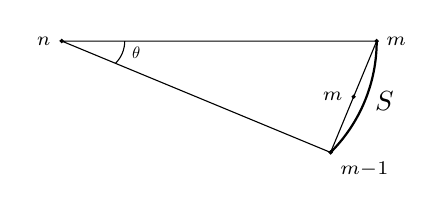
\begin{tikzpicture}
    \begin{scope}[scale = 2]
        \def\r{1}\def\smallr{.2}
        \def\thetai{-45}\def\thetaf{0}\def\thetam{180}
        \draw
            (
                {(1-\smallr)*\r*cos(\thetam) + \smallr*\r*cos(\thetaf)},
                {(1-\smallr)*\r*sin(\thetam) + \smallr*\r*sin(\thetaf)}
            ) arc (\thetaf:\thetai:\smallr) node[midway, right]{\scalebox{.6}{$\mathtt{\theta}$}};
        \draw[cap = round]
            ({\r*cos(\thetaf)}, {\r*sin(\thetaf)})--
            ({\r*cos(\thetam)}, {\r*sin(\thetam)})--
            ({\r*cos(\thetai)}, {\r*sin(\thetai)})--cycle;
        \draw[thick] ({\r*cos(\thetai)}, {\r*sin(\thetai)}) arc (\thetai:\thetaf:\r) node[midway, right]{$S$};
        \draw[fill = black] ({\r*cos(\thetaf)}, {\r*sin(\thetaf)}) circle (.01) node[right]{$\xvec_m$};
        \draw[fill = black] ({\r*cos(\thetai)}, {\r*sin(\thetai)}) circle (.01) node[below right]{$\xvec_{m-1}$};
        \draw[fill = black] ({\r*cos(\thetam)}, {\r*sin(\thetam)}) circle (.01) node[left]{$\bzhe_n$};
        \draw[fill = black]
            (
                {.5*\r*cos(\thetaf) + .5*\r*cos(\thetai)},
                {.5*\r*sin(\thetaf) + .5*\r*sin(\thetai)}
            ) circle (.01) node[left]{$\bzhe_m$};
    \end{scope}
\end{tikzpicture}
\end{figure}
\noindent Letting $\Re(\star)$ denote the real part of a complex number, and noting that $r_m = \absl{\xvec_m - \bzhe_n}$, we have that\footnote{\cite{abramowitz1965handbook} \textsc{Abramowitz} \& \textsc{Stegun}, p.67, eq.4.1.2}
\[
    \ln{r} = \Re\big( \ln{(\ezh - \bzhe_n)} \big), \quad \ezh = x + iy.
\]
Now,
\[
    \int_{S} \nhat\cdot\nabla\ln{r}\,\dee S = \Re \int_{S} \frac{i}{\ezh - \bzhe_n} \,\dee\ezh.
\]
Evaluating the integral at the points $\xvec_{m}$ and $\xvec_{m - 1}$, and using the fact that $\ln{\ezh} = \ln{\absl{\ezh}} + i\arg{\ezh}$, we get that
\[
    \int_{S} \nhat \cdot \nabla \ln{r} \,\dee S = \Theta_{n,m-1} - \Theta_{n,m} \equiv - \Thetatt,
\]
where $\Theta_{n,m} = \arg{(\xvec_m - \bzhe_n)}$.
We note that this contribution to the discrete integral equation is exact, and it is the assumption that $\phi$ is constant along the line segment $S_m$ that causes inaccuracy.

\subsection{Quadrature Methods}
To integrate the logarithm, we employ a so-called \textsc{Gauss} quadrature method of the second order.
This method has us map the domain of integration to the one dimensional unit circle,\footnote{\cite{abramowitz1965handbook} \textsc{Abramowitz} \& \textsc{Stegun}, pp.779 \& 887}
\[
    \int_{a}^{b} y(x) \,\dee x \mapsto \int_{-1}^{1} \eta(\xi) \,\dee\xi,
\]
where
\[
    x = \frac{b - a}{2} \xi + \frac{a + b}{2}, \qquad \eta(\xi) \equiv \frac{b - a}{2} y(x).
\]
This latter integral we approximate by
\[
    \sum_{k = 1}^{N} w_k \eta(\xi_k), \quad w_k = \frac{2}{\big(1 - {\xi_k}^2\big){\big(\legendre_{N}^{\prime}(\xi_k)\big)}^2},
\]
Where $\legendre_N$ is the $N$\textsuperscript{th}-degree \textsc{Legendre} polynomial, and $\xi_k$ are its $N$ zeros.
Setting $N = 2$, and recalling the three first \textsc{Legendre} polynomials,
\[
    \legendre_0(\xi) = 1, \quad \legendre_1(\xi) = \xi, \quad \legendre_2(\xi) = \frac{3\xi^2 - 1}{2},
\]
We find that $w_1 = 1$ and $w_2 = 1$, and $\xi_k = \pm \sfrac{1}{\sqrt{3}}$.
Recalling the logarithm rule $\ln{(x^\alpha)} = \alpha\ln{x}$, we have that
\[
    \int_{S_m} \ln{r} \,\dee S \approx \frac{1}{2}\sum_{k = 1}^{2} \frac{\absl{\xvec_m - \xvec_{m-1}}}{2}\ln{{\absl{\xvec_{m}^{\prime} - \bzhe_n}}^2},
\]
where
\[
    \xvec_{m}^{\prime} = \frac{\xvec_{m} + \xvec_{m-1}}{2} + \frac{{(-1)}^k (\xvec_{m} - \xvec_{m-1})}{2\sqrt{3}}.
\]
We usually label the tensor collection of such integrals $\mathtt{h}$.

\subsection{The Discrete Integral Equation}
We note that $\partial_{\nhat}\phi_m$ has three modes corresponding to each of the Cartesian unit vectors, and that the subscript $m$ denotes evaluation at that indexed node, and likewise with the rotational normal vectors.
Since we consider here a Galilean coordinate system---moving with the geometry---the $\phi$ here represent velocity potentials due to geometry motion with unit velocity some mode.\footnote{\cite{newman2018marine} \textsc{Newman}, pp.143--144}
It is meant here, then, that $\partial_{\nhat} \phi_m = n_i$, where $n_i$ is whichever normal vector component.
The integral equation is then given as follows.
\[
    -\pi \phi_n - \sum_{m = 1}^{N} \phi_m \Thetatt_{n,m} = \sum_{m = 1}^{N} \partial_{\nhat} \phi_m \mathtt{h}_{n,m}.
\]

\subsection{Added Mass}
The added mass tensor $\addedmass$ may be similarly approximated.
\[
    \addedmass = \varrho \int_{\partial\Omega} \phi_j n_i \,\dee S = \varrho\sum_{m = 1}^{N} \absl{\xvec_{m} - \xvec_{m-1}} {\phi_j}_m {n_i}_m
\]